\documentclass{beamer}
\usepackage{tikz}
\usetikzlibrary{matrix,backgrounds}

\begin{document}

\begin{frame}[fragile]

\begin{center}
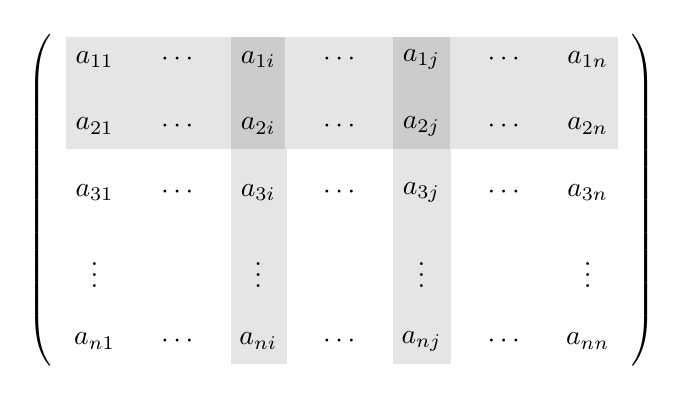
\begin{tikzpicture}
\matrix (m) [
    matrix of math nodes,
    left delimiter={(}, right delimiter={)},
    column sep=10pt, row sep=8pt,
    nodes={minimum width=1.6em, minimum height=1.6em, anchor=center}
]
{
a_{11} & \cdots & a_{1i} & \cdots & a_{1j} & \cdots & a_{1n} \\
a_{21} & \cdots & a_{2i} & \cdots & a_{2j} & \cdots & a_{2n} \\
a_{31} & \cdots & a_{3i} & \cdots & a_{3j} & \cdots & a_{3n} \\
\vdots &        & \vdots &        & \vdots &        & \vdots \\
a_{n1} & \cdots & a_{ni} & \cdots & a_{nj} & \cdots & a_{nn} \\
};

\begin{pgfonlayer}{background}
  % first two rows, full width -- light gray
  \fill[gray!20] (m-1-1.north west) rectangle (m-2-7.south east);
  % columns i and j, full height -- light gray
  \fill[gray!20] (m-1-3.north west) rectangle (m-5-3.south east);
  \fill[gray!20] (m-1-5.north west) rectangle (m-5-5.south east);
  % the four overlap cells -- darker gray, drawn on top
  \fill[gray!40] (m-1-3.north west) rectangle (m-2-3.south east);
  \fill[gray!40] (m-1-5.north west) rectangle (m-2-5.south east);
\end{pgfonlayer}
\end{tikzpicture}
\end{center}

\end{frame}

\end{document}
